\chapter{Model inference for production systems}
\label{sec:modelinf:prodsystems}

In this chapter, we introduce \emph{Autofunk v2} following by
\emph{Autofunk v3}. This is our passive model inference
framework, improving \emph{Autofunk v1}'s capabilities, and
focused on inferring models of production systems. It combines
model inference, machine learning, and expert systems to infer \\

\minitoc

\pagebreak

\section{Introduction}

In the Industry, building models for production systems,
\emph{i.e.} event-driven systems that run in production
environments and are distributed over several devices and
sensors, is frequent since these are valuable in many situations
like testing and fault diagnosis for instance. Models may have
been written as storyboards or with languages such as the Unified
Modeling Language (UML) or even more formal languages. Usually,
these models are designed when brand-new systems are built. It
has been pointed out by our industrial partner that production
systems have a life span of many years, up to 20 years, and are
often incrementally updated, but their corresponding models are
not.  This leads to a major issue which is to keep these models
up to date and synchronized with the respective systems. This is
a common problem with documentation in general, and it often
implies rather under-specified or not documented systems that no
one wants to maintain because of lack of understanding.

In this chapter, we focus on this problem for production systems
that exchange thousands of events a day. Several approaches have
already been proposed for different types of systems.  Yet, we
noticed that these approaches were not tailored to support
production systems. From the literature,
\crossref{sec:related}{sec:related:modelinf}, we deduced the
following key observations:

\begin{itemize}
    \item Most of the existing model inference approaches give
        approximate models capturing the behaviors of a system
        and more. In our context, we want exact models that could
        be used for regression test case generation, and fault
        diagnosis. We define exactness with the
        \emph{trace-inclusion} and \emph{trace-equivalence}
        relations given in \cite{petrenko06};

    \item Applying active inference on running systems is
        complicated since these must not be disrupted (otherwise
        it may lead to severe damages on the production
        machines), but also because we cannot rely on any oracle
        or teacher;

    \item Production systems exchange thousands and thousands of
        events a day. Again, most of the model inference
        approaches cannot take such a huge amount of information
        to build models. We need a solution that is scalable.
\end{itemize}

Based on these observations, we propose a pragmatic \emph{passive
model inference} approach that aims at building formal models
describing functional behaviors of a system. Our goal is to
quickly build exact models from large amounts of production
events.  Furthermore, execution speed takes an important place
for building up to date models. Such models could also be used
for diagnosis every time an issue would be experienced in
production.  The strong originality of our approach lies in the
combination of two domains for model inference: model-driven
engineering and expert systems. We consider formal models and
their definitions to infer models by means of different
transformations. But we also take into consideration the
knowledge of human experts captured by expert systems. A part of
our approach is based upon this notion of knowledge implemented
with inference rules. We reuse what worked well for web
applications and enhance many parts of our framework to come up
with a better version of our \textit{Autofunk} framework, which
is presented throughout this thesis.

In the following section, we describe the context in which this
work has been conducted. In Section
\ref{sec:modelinf:prodsystems:autofunk}, we present
\textit{Autofunk} for Michelin's production systems along with a
case study. Section \ref{sec:modelinf:usability} highlights our
work on improving usability of the generated models.  We give our
results in Section \ref{sec:modelinf:prodsystems:results}. We
highlight an improvement made on our framework in Section
\label{sec:modelinf:prodsystems:better-segmentation}, which is
part of \emph{Autofunk v3}. We conclude on this chapter in
Section \ref{sec:modelinf:prodsystems:conclusion}.

\textbf{Publications.} This work has been published in the
Proceedings of Formal Methods 2015 (FM'15)
\cite{DBLP:conf/fm/DurandS15}, and in the Proceedings of the 9th
International Conference on Distributed Event-Based Systems
(DEBS'15) \cite{DBLP:conf/debs/SalvaD15}.

\section{Context at Michelin}
\label{prodsys:context}

Michelin is a worldwide tire manufacturer and designs most of its
factories, production systems, and software by itself.  Like
many other industrial companies, Michelin follows the \emph{Computer
Integrated Manufacturing} (CIM) approach \cite{rehg2004computer},
using computers and software to control the entire manufacturing
process. In this thesis, we focus on the Level 2 of the CIM
approach, \emph{i.e.} all the applications that monitor and control
several production devices and \emph{points}, \emph{i.e.}
locations where a production line branches into multiple lines,
in a workshop. In a factory, there are different \emph{workshops}
for each step of the tire building process. At a workshop level,
we observe a continuous stream of products from specific entry
points to a finite set of exit points, \emph{i.e.} where products
go to reach the next step of the manufacturing process, and
disappear of the workshop frame in the meantime, as shown in
Figure \ref{fig:workshop-annotated}.  Depending on the workshops,
products can stay in this frame for days up to several weeks.
Indeed, a workshop may contain storage areas where products can
stay for a while, depending on the production campaigns or needs
for instance.  Thousands and thousands of \emph{production
events} are exchanged among the industrial devices of the same
workshop every day, allowing some factories to build over 30,000
tires a day.

\begin{figure}[ht]
    \begin{center}
        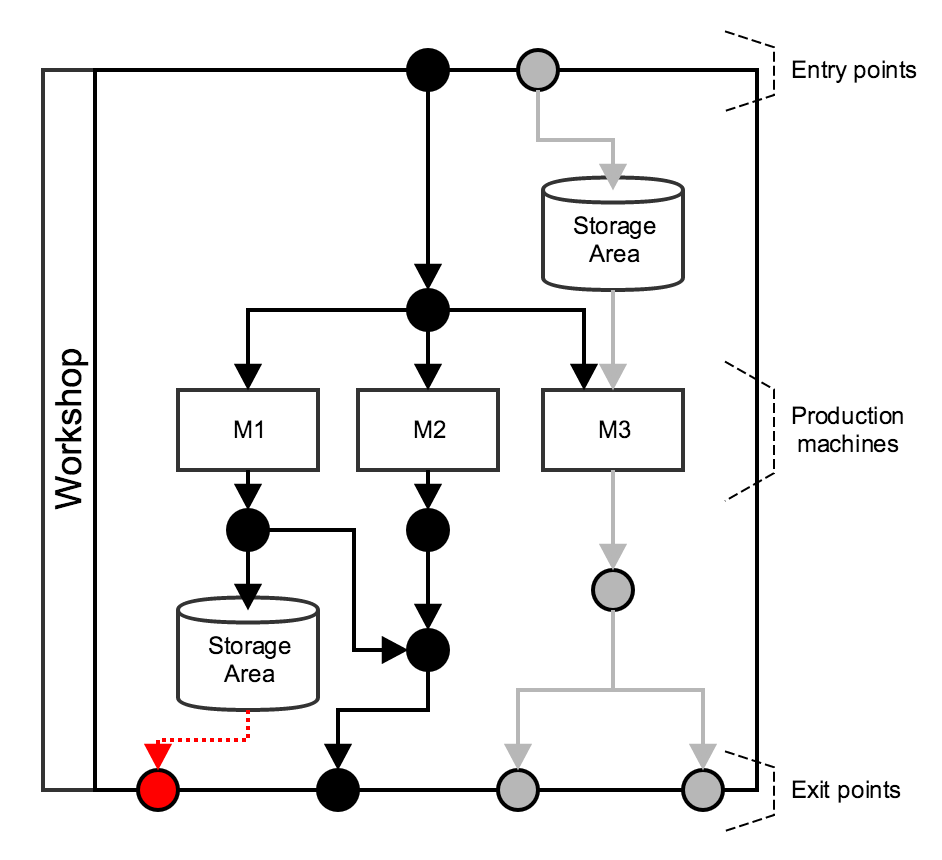
\includegraphics[width=1.0\linewidth]{figures/workshop-annotated.png}
    \end{center}

    \caption{A workshop owns a set of known entry and exit
    points. A continuous stream of products starts from known
    entry points, and ends at known exit points. This figure
    shows two production lines: the grey line having two exit
    points (represented by the circles), and the black one having
    only one real exit point, not two. The red dotted line
    represents a false-positive here, which is a problem we have
    to take into account while detecting (entry and) exit
    points.}
    \label{fig:workshop-annotated}
\end{figure}

Although there is a finite number of applications, each has
different versions deployed in factories all over the world,
potentially highlighting even more different behaviors and
features. Even if a lot of efforts are put into standardizing
applications and development processes, different programming
languages and different frameworks are used by development
teams, making difficult to focus on a single technology. Last
but not least, the average lifetime of these applications is 20
years. This set is large and too disparate to apply conventional
testing techniques, yet most of the applications exchange events
using dedicated custom internal protocols.

Our industrial partner needs a safe way to infer up to date
models, independent of the underlying technical details, and
without having to rely on any existing documentation.
Additionally, Michelin is interested in building regression test
suites to decrease the time required to deploy or upgrade
systems. We came up to the conclusion that, in order to target
the largest part of all Michelin's Level 2 applications, taking
advantage of the production events exchanged among all devices
would be the best solution, as it would not be tied to any
programming language or framework, and these events contain all
information needed to understand how a whole industrial system
behaves in production. All these events are collected
synchronously through a (centralized) logging system. Such a
system logs all events with respect to their order, and does not
miss any event.  From these, we chose not to use extrapolation
techniques to infer models, meaning our proposal generates
exact models, exclusively describing what really happens
in production.

This context leads to some assumptions that have been considered
to design our framework:

\begin{itemize}
    \item \textbf{Black-box systems:} production systems are seen as
        black-boxes from which a large set of production events can
        be passively collected. Such systems are compound of
        production lines fragmented into several devices and sensors.
        Hence, a production system can have several entry and exit
        points. We denote such a system by $\mathit{Sua}$ (\emph{system
        under analysis});

    \item \textbf{Production events:} an event of the form
        $a(\alpha)$ must include a distinctive label $a$ along with a
        parameter assignment $\alpha$. Two events $a(\alpha_1)$ and
        $a(\alpha_2)$ having the same label $a$ must own assignments
        over the same parameter set. The events are ordered and
        processed with respect to this order;

    \item \textbf{Traces identification:} traces are sequences of
        events $a_1(\alpha_1) \cdot \dots \cdot a_n(\alpha_n)$. A
        trace is identified by a specific parameter that is
        included in all event assignments of the same trace. This
        identifier is denoted by $pid$ and identifies products,
        \emph{e.g.}, tires at Michelin.  Besides this, event
        assignments include a time stamp to sort the events into
        the traces.
\end{itemize}

%%%%%%%%%%%%%%%%%%%%%%%%%%%%%%%%%%%%%%%%%%%%%%%%%%%%%%%%%%%%%%%%%

\section{\textit{Autofunk}'s models generator revisited}
\label{sec:modelinf:prodsystems:autofunk}

In this section, we introduce our framework \textit{Autofunk v2},
whose main architecture is depicted in Figure
\ref{fig:prodsystems:autofunk-overview}. This new version also
contains different modules (in grey in the figure): four modules
are dedicated to build models, and an optional one can be used to
derive more abstract and readable models.

\begin{figure}[ht]
    \begin{center}
        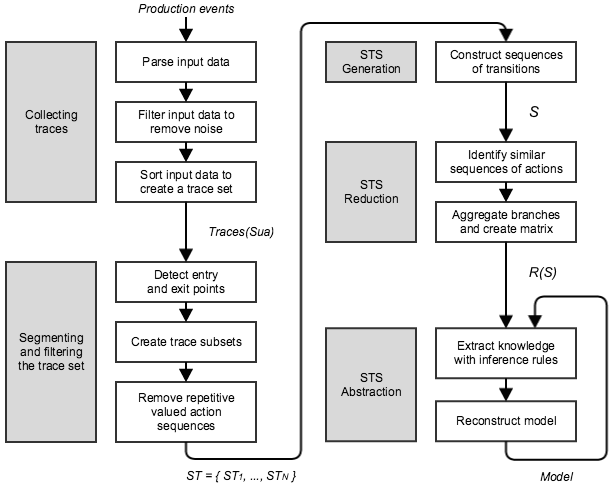
\includegraphics[width=1.0\linewidth]{figures/autofunk.png}
    \end{center}

    \caption{Overview of \textit{Autofunk} revisited with the different
    modules in grey along with their corresponding steps. The last
    module (STS abstraction) is optional.}
    \label{fig:prodsystems:autofunk-overview}
\end{figure}

Here, we consider \textit{Symbolic Transition Systems} (STSs) as
models for representing production system behaviors. As reminder,
STSs are state machines incorporating actions (\emph{i.e.} events
in this context), labeled on transitions, that show what can be
given to and observed on the system. In addition, actions are
tied to an explicit notion of data. A formal definition can
be found in \crossref{sec:related}{sec:definitions:sts}.
The innovation of this framework lies in the combination of the
notion of expert systems with the STS formalism: the STS
representation, operators and transformations, are expressed
with deduction rules, and the knowledge of a human expert of a
system can be transcribed with inference rules.
\textit{Autofunk v2} combines both domains in such a way that
each model modification can be expressed and implemented with a
rule.  As a consequence, the data collections handled by
\textit{Autofunk} are always expressed with knowledge bases
(Events, Actions, Traces, STSs, etc.) on which rules are applied
to infer models. Given a system $\mathit{Sua}$ and a set of
production events, \textit{Autofunk} builds \emph{trace-included}
models, \emph{i.e.} the traces of a model $\EuScript{S}$ are
included in the traces of $\mathit{Sua}$.

\begin{figure}[ht]
\begin{framed}
\begin{BVerbatim}
17-Jun-2014 23:29:59.00|INFO|New File

17-Jun-2014 23:29:59.50|17011|MSG_IN  [nsys: 1] \
  [nsec: 8] [point: 4] [pid: 1]

17-Jun-2014 23:29:59.61|17021|MSG_OUT [nsys: 1] \
  [nsec: 8] [point: 4] [tpoint: 8] [pid: 1]

17-Jun-2014 23:29:59.70|17011|MSG_IN  [nsys: 1] \
  [nsec: 8] [point: 4] [pid: 2]

17-Jun-2014 23:29:59.92|17021|MSG_OUT [nsys: 1] \
  [nsec: 8] [point: 4] [tpoint: 8] [pid: 2]
\end{BVerbatim}
\end{framed}

\caption{An example of some production events. Each event is
time-stamped, has a label (\emph{e.g.}, $17011$), and may own
assignments of variables (\emph{e.g.}, $nsys$).}
\label{fig:rawdatum}
\end{figure}

To explain how \textit{Autofunk v2} works with production
systems, we consider a case study based upon the example of
Figure \ref{fig:rawdatum}. It depicts simplified production
events similar to those extracted from Michelin's logging system.
$INFO$, $17011$, and $17021$ are labels along with assignments of
variables \emph{e.g.}, $nsys$, which indicates an industrial
device number, and $point$, which gives the product position.
Real events own around 20 parameters in average. Such a format is
specific to Michelin but other kinds of events could be
considered by updating the first module of \textit{Autofunk}.  In
this example, each line represents an event that happened in the
system. This format has been borrowed from Michelin's logging
system, hence its special formatting. It is worth mentioning that
the first line of this set is an event that is tied to the
logging system, not the production system we are interested in.

\subsection{Production events and traces}
\label{part3:collecting}

\textit{Autofunk} takes production events as input from a system
under analysis $\mathit{Sua}$. To avoid disrupting the (running)
system $\mathit{Sua}$, we do not instrument the industrial
equipment composing the whole system. Everything is done offline
with a logging system or with monitoring. We start by formatting
these events to obtain a set of events of the form $a(\alpha)$
with $a$ a label, and $\alpha$ a parameter assignment. We call
these formatted events, \textit{valued events}. Valued events are
similar to valued actions (as in Chapter
\ref{sec:modelinf:webapps}) except that this term is more
accurate in our industrial context.  Performing such a step
allows to collect productions events from various sources, and
still be able to perform the next steps in a unique manner.

In this set, some of these valued events may be irrelevant.  For
instance, some events may capture logging information and are not
part of the functioning of the system. In Figure
\ref{fig:rawdatum}, the event having the type $INFO$
belongs to this category and can be safely removed. Filtering is
achieved by an expert system and inference rules. Here again, a
human expert knows which events should be filtered out, and
inference rules offer a natural way to express his knowledge. On
top of that, expert systems also offer fast processing in this
situation. We use inference rules of the form:

\textit{When $a(\alpha)$, condition on $a(\alpha)$, then
retract($a(\alpha)$)}.

The remaining valued events are time-ordered to produce an
initial set of traces denoted by $Traces(Sua)$. Figure
\ref{fig:tsua} illustrates this set obtained from the events of
Figure \ref{fig:rawdatum}.

\begin{figure}[ht]
\begin{framed}
    $Traces(Sua) = \{
    (17011(nsys:=1,nsec:=8,point:=4,pid:=1)\text{ }
    17021(nsys:=1,nsec:=8,point:=4,tpoint:=8,pid:=1))$,
    $(17011(nsys:=1,nsec:=8,point:=4,pid:=2)\text{ }
    17021(nsys:=1,nsec:=8,point:=4,tpoint:=8,pid:=2)) \}$
\end{framed}

\caption{Initial trace set $Traces(Sua)$ based on the events
given in Figure \ref{fig:rawdatum}.}
\label{fig:tsua}
\end{figure}

Figure \ref{fig:removalrules} shows two concrete rules applied to
Michelin systems. These two rules are written with the Drools
formalism, already introduced in the previous chapter. The first
rule removes valued events including the $INFO$ parameter,
which do not contain any business value. The variable
$\$valued\_event$ is a valued event (instance of $ValuedEvent$),
containing parameter assignments ($Assign$ attribute) that can be
accessed using the following notation: $Assign.foo$ where $foo$
is a name and the result its corresponding value.

The second rule in Figure \ref{fig:removalrules} removes valued
events extracted from very specific events, \emph{i.e.} those
whose $key$ matches a pattern and having a $inc$ value that is
not equal to $1$.  To fully understand the syntax of this rule,
one has to know that when there is no logical connective between
the conditions, it defaults to a conjunction.  Such a rule has
been given by a Michelin expert and allows to remove some
duplicate events.  In the context of Michelin, we use four
inference rules to remove all irrelevant events.

\begin{figure}[ht]
\begin{framed}
\begin{BVerbatim}
rule "Remove INFO events"
when:
  $valued_event: ValuedEvent(Assign.type == TYPE_INFO)
then
  retract($valued_event)
end
\end{BVerbatim}
\end{framed}

\begin{framed}
\begin{BVerbatim}
rule "Remove events that are repeated"
when
  $valued_event: ValuedEvent(
    Assign.key matches "KEY_NAME_[0-9]+",
    Assign.inc != null,
    Assign.inc != "1"
  )
then
  retract($valued_event)
end
\end{BVerbatim}
\end{framed}

\caption{An example of inference rules used for filtering
purpose. It contains two rules: the first one is used to remove
events including the $INFO$ label, the second one is used to omit
events that are repeated.}
\label{fig:removalrules}
\end{figure}

From this filtered valued event base, we reconstruct the
corresponding traces from the trace identifier $pid$, present in
each valued event, and time stamps. We call the resulting trace
set $Traces(Sua)$:

\begin{definition}[$Traces(Sua)$]
    Given a system under analysis $\mathit{Sua}$, $Traces(Sua)$
    denotes its \emph{formatted trace set}. $Traces(Sua)$
    includes traces of the form $(a_1,\alpha_1) \cdot \dots \cdot
    (a_n,\alpha_n)$ such that $(a_i,\alpha_i)_{(1 \leq i \leq
    n)}$ are (ordered) valued events having the same identifier
    assignment.

	\label{def:structuredtrace}
\end{definition}

We can now state that a STS model $\EuScript{S}$ is said
\emph{trace-included} if and only if $Traces(\EuScript{S})
\subseteq Traces(Sua)$ as defined in \cite{petrenko06}.

\subsection{Trace segmentation and filtering}
\label{sec:modelinf:prodsystems:segmentation}

In Section \ref{prodsys:context}, we indicated that products
could stay in a workshop for days and even weeks. From our point
of view, this means that we can likely collect partial
executions, \emph{i.e.} events belonging to products that were present
in the workshop we are observing before we start to collect any
events. We can determine which product was present in the
workshop before by retrieving the first event tied to it.
If the physical location of this event is not one of the known
entry points of the workshop, then the product was there before.
In a similar manner, we are able to retrieve \emph{incomplete
executions} related to the end of the collection, \emph{i.e.} the
events tied to products that did not reach any of the known exit
points of the workshop.

We define a \textit{complete trace} as a trace containing all
events expressing the path taken by a product in a production
system, from the beginning, \emph{i.e.} one of its entry points,
to the end, \emph{i.e.} one of its exit points. In the trace set
$Traces(Sua)$, we do not want to keep incomplete traces,
\emph{i.e.}  traces related to products which did not pass
through one of the known entry points or moved to the next step
of the manufacturing process using one of the known exit points.

\begin{definition}[Complete traces]
    Let $\mathit{Sua}$ be a system under analysis and
    $Traces({Sua})$ be its trace set. A trace $t=a_1(\alpha_1)
    \cdot \dots \cdot a_n(\alpha_n) \in Traces({Sua})$ is said
    \emph{complete} if and only if $\alpha_1$ includes an
    assignment $(point:=val1)$, which denotes an entry point of
    $\mathit{Sua}$, and $\alpha_n$ includes an assignment
    $(point:=val2)$, which denotes an exit point.

    The \emph{complete traces} of $\mathit{Sua}$ are denoted by
    $CTraces({Sua}) \subseteq Traces({Sua})$.
\end{definition}

We also chose to split $Traces(Sua)$ constructed in the previous step
into subsets $ST_i$, one for each entry point of the system under
analysis $\mathit{Sua}$. Later, every trace set $ST_i$ shall give
birth to one model, describing all possible behaviors starting
from its corresponding entry point.

This module performs these two steps, which are summarized in
Algorithm \ref{algo_traces}. It starts by splitting $Traces(Sua)$
into several trace sets $ST_i$, one for each entry point of the
system $\mathit{Sua}$, and then removes incomplete traces. Since
we want a framework as flexible as possible, we chose to perform
a statistical analysis on $Traces(Sua)$ aiming at automatically
detecting the entry and exit points.  In Michelin systems, the
parameter $point$ stores the product physical location and can be
used to deduce the entry and exit points of the systems.
This analysis is performed on the assignments $(point:=val)$
found in the first and last valued events of the traces of
$Traces(Sua)$ since $point$ captures the product physical
location and especially the entry and exit points of $\mathit{Sua}$.
We obtain two ratios $Rinit(point:=val1)$ and
$Rfinal(point:=val2)$.  Based on these ratios, one can deduce the
entry point set $POINT_{init}$ and the exit point set
$POINT_{final}$ if $Traces(Sua)$ is large enough. Pragmatically,
we observed that the traces collected during one or two days are
not sufficient because they do not provide enough differences
between the ratios. In this case, we assume that the number of
entry and exit points, $N$ and $M$, are given and we keep the
first $N$ and $M$ ratios only. On the other hand, a week offers
good results. We chose to set a fixed yet configurable
minimum limit to 10\%. Assignments $(point:=val)$ having a ratio
below this limit are not retained. Then, for each assignment
$\alpha_i=(point:=val1)$ in $POINT_{init}$, we construct a trace
set $ST_i$ such that a trace of $ST_i$ has a first valued event
including the assignment $\alpha_i$, and ends with a valued event
including an assignment $(point:=val2)$ in $POINT_{final}$. We
obtain the set $ST=\{ST_1,...,ST_N\}$ with $N$ the number of
entry points of the system $\mathit{Sua}$.

In our straightforward example, we obtain one trace set
$ST_1=Traces(Sua)$.

Thereafter, \textit{Autofunk} scans the traces in $ST$ and tries
to detect repetitive patterns $p,\dots,p$. If it finds a trace
$t$ having a repetitive pattern $p$ and another equivalent trace
including this pattern $p$ once, then $t$ is removed since we
suppose that $t$ does not express a new and interesting behavior.
Here, traces are removed rather than deleting the repetitive
patterns to prevent from modifying traces and to keep the
\emph{trace inclusion} \cite{petrenko06} property between
$CTraces(Sua)$ and $Traces(Sua)$.  In Algorithm
\ref{algo_traces}, two traces $t=\sigma_1 p,\dots,p \sigma_n$ and
$t'=\sigma_1 p' \sigma_n$ are said equivalent if the patterns
$p$, $p'$ and the sub-sequences are equivalent, denoted by the
$\sim_{(pid)}$ notation:

\begin{definition}[The $\sim_{(pid)}$ relation]
    Let $p$ be a pattern of a trace $t$ and $p'$ be a pattern of
    a trace $t'$. We denote by $\sim{(pid)}$ the relation that
    defines the equivalence between $t$ and $t'$, and we write
    $t \sim_{(pid)} t'$ if and only if $t$ and $t'$ have the same
    successive valued events after having removed the assignments
    of the variable $pid$.
\end{definition}

At the end we obtain the complete trace set $CTraces(Sua)$.

\begin{algorithm}[h]
	\SetKwInOut{Input}{input}
	\SetKwInOut{Output}{output}

  \Input{$Traces(Sua)$,\\optionally entry point number $N$ and/or exit point number $M$}
  \Output{$CTraces(Sua)=\{ST_1,...,ST_n\}$}

\BlankLine
BEGIN\;
\emph{Step 1. $Traces(Sua)$ segmentation}

\ForEach{$t=(a_1,\alpha_1)...(a_n,\alpha_n) \in Traces(Sua)$} {
$Rinit((point:=val)\subset \alpha_1)++$\;
$Rfinal((point:=val2)\subset \alpha_n)++$\;
}
$POINT_{init}=\{(point:=val) \mid Rinit((point:=val))>10$\% or belongs to the N highest ratios$\}$\;
$POINT_{final}=\{(point:=val) \mid Rfinal((point:=val))>10$\% or belongs to the M highest ratios$\}$\;
\BlankLine

\ForEach{$\alpha_i=(point:=val) \in POINT_{init}$} {
	$ST_i=\{a1(\alpha_1)...an(\alpha_n)\in Traces(Sua) \mid \alpha_i\subset \alpha_1, \exists (point:=val2)\subset \alpha_n, (point:=val2)\in POINT_{final}    \}$\;
}
$ST:=\{ST_1,...,ST_N\}$\;

\BlankLine
\emph{Step 2. trace filtering}

\ForEach{$t=\sigma_1p...p\sigma_n\in ST$} {
	\If{ $\exists t'=\sigma_1'p'\sigma_n'\in ST$ such that $p\sim_{(pid)}p'$, $\sigma_1\sim_{(pid)}\sigma_1'$, $\sigma_n\sim_{(pid)}\sigma_n'$ }
	{
		$ST:= ST/ \{  t \}$\;
	}


	}

    $CTraces(Sua) := ST$

END\;

\caption{Trace segmentation algorithm}
\label{algo_traces}
\end{algorithm}

\subsection{STS generation}
\label{sec:modelinf:prodsystems:generation}

One model is then built for each trace set $ST_i \in
CTraces(Sua)$ by reusing the technique introduced in
\crossref{sec:modelinf:webapps}{sec:iosts-gen}. Given a set
$ST_i$, a first STS, denoted by $\EuScript{S}_i$, is built in a
simple yet quick manner. Each trace of $ST_i$ is completed to
derive a set of runs. A run is an alternate sequence of states
and events. Given a trace $t$ in $ST_i$, states, which are
unique, are injected before and after each event of $t$. States
must be unique to keep the ordering of the events in the runs,
and to prevent merging different behaviors in the model.  The
initial state is an exception though as it is shared by all the
runs. The model $\EuScript{S}_i$ is obtained by transforming runs
into sequences of transitions that are then joined together.

The translation of $ST_i$ into a run set denoted by $Runs_i$ is done
by completing traces with states. Each run starts by the same
initial state $(l0,v_\emptyset)$ with $v_\emptyset$ the empty
assignment. Then, new states are injected after each event.
$Runs_i$ is formally given by the following definition:

\begin{definition}[Structured runs]
  Let $ST_i$ be a complete trace set obtained from
  $\mathit{Sua}$. We denote by $Runs_i$ the set of runs derived from
  $ST_i$ with the following inference rule:

  \begin{center}
    {\Large
    $\frac{\sigma_{k(1\leq k \leq n)}=(a_1,\alpha_1)...(a_n,\alpha_n) \in ST_i}
    {(l0,v_\emptyset) (a_1,\alpha_1) (l_{k1},v_\emptyset) \dots (l_{kn-1},v_\emptyset) (a_n,\alpha_n) (l_{kn},v_\emptyset) \in Runs_i}$
    }
  \end{center}
\end{definition}

The above definition preserves trace inclusion \cite{petrenko06}
between $Runs_i$ and $Traces(Sua)$ because we only inject states
between valued events, and we can deduce the following
proposition:

\begin{proposition}
Let $ST_i$ be a trace set obtained from $\mathit{Sua}$. We have
$Traces(Runs_i) \subseteq Traces(Sua)$.
\end{proposition}

The runs of $Runs_i$ have states that are unique except for the
initial state $(l0,v_\emptyset)$. We defined such a set to
ease the process of building a STS having a tree structure.  Runs
are transformed into STS paths that are assembled together by
means of a disjoint union. The resulting STS forms a tree
compound of branches starting from the location $l0$. Parameters
and guards are extracted from the assignments found in valued
events:

\begin{definition}[Run set to STS]
  Given a run set $Runs_i$, $\EuScript{S}_i=<L_{\EuScript{S}_i},
  l0_{\EuScript{S}_i},V_{\EuScript{S}_i}, V0_{\EuScript{S}_i},
  I_{\EuScript{S}_i},\\
  \Lambda_{\EuScript{S}_i},\rightarrow_{\EuScript{S}_i}>$ is the
  STS expressing the behaviors found in $Runs_i$ such that:

	\begin{itemize}
    \item $L_{\EuScript{S}_i}= \{l_i \mid \exists r\in Runs_i,
      (li,v_\emptyset)$ is a state found in $r\}$;

    \item $l0_{\EuScript{S}_i} = l0$ is the initial location
      such that $\forall r \in Runs_i$, $r$ starts with
      $(l0,v_\emptyset)$;

    \item $V_{\EuScript{S}_i}=\emptyset$, $V0_{\EuScript{S}_i}=v_\emptyset$;

    \item $\rightarrow_{\EuScript{S}_i}$ and
      $\Lambda_{\EuScript{S}_i}$ are defined by the following
      inference rule applied to every element $r\in Runs_i$:
	\end{itemize}

  \begin{center}
    {\Large
    $\frac{(l_i,v_\emptyset) (a_i,\alpha_i) (l_{i+1},v_\emptyset)
    \in r, p=\{x \mid (x:=v)\in \alpha_i \}, G_i=\displaystyle
  \bigwedge_{(x:=v)\in \alpha_i}x==v}{l_i \xrightarrow{a_i(p),G_i,id_V}_{\EuScript{S}_i} l_{i+1}}$
    }
  \end{center}


  \label{def:runset_to_sts}
\end{definition}

We obtain a model having a tree structure and whose traces are
equivalent \cite{petrenko06} to those of $CTraces(Sua)$ because
each run is transformed into a unique STS path, only sharing a
common initial location $l0$, and for each path, the guard
corresponds to the conjunction of the assignments of the
variables found in the trace, which is important to avoid
over-approximation. This is captured by the proposition below. At
this point, production events are called actions of the STS.

\begin{proposition}
    Let $ST_i$ be a complete trace set obtained from
    $\mathit{Sua}$, and $Runs_i$ the set of runs derived from
    $ST_i$.
    We have $Traces(Runs_i) = CTraces(Sua) \subseteq Traces(Sua)$.

    \label{}
\end{proposition}

Figure \ref{fig:firstmodel} depicts the model obtained from the
traces given in Figure \ref{fig:tsua}. Every initial trace is now
represented as a STS branch. Parameter assignments are modeled
with constraints over transitions, called \textit{guards}.

\begin{figure}[ht]
    \begin{center}
        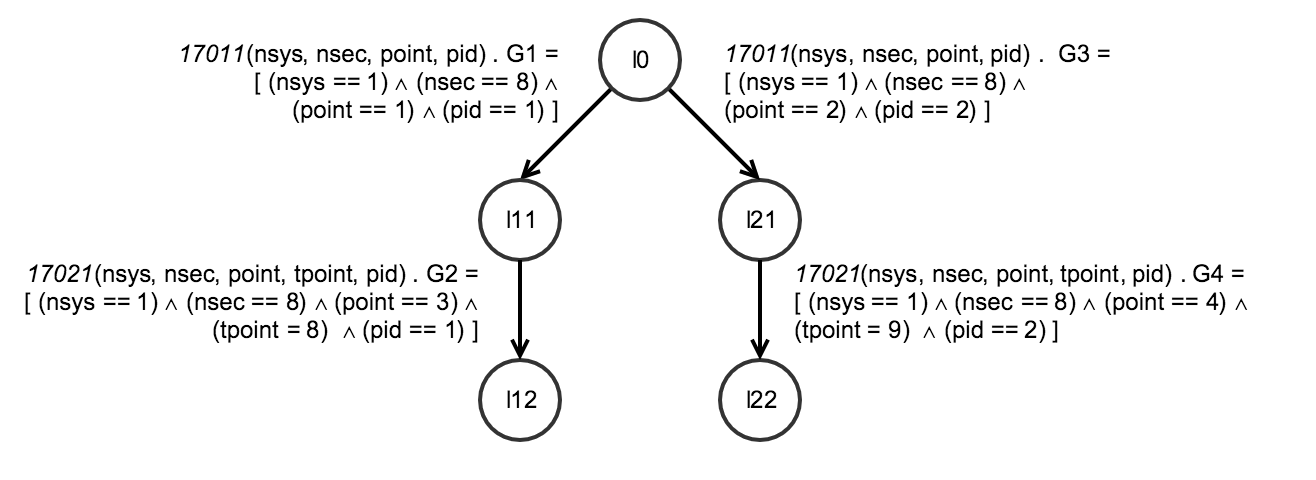
\includegraphics[width=1.0\linewidth]{figures/STS1.png}
    \end{center}

  \caption{First generated Symbolic Transition System model,
  based on the traces given in Figure \ref{fig:tsua}.}
  \label{fig:firstmodel}
\end{figure}

This STS expresses the behaviors found in $Traces(Sua)$ but in a
slightly different manner. Trace inclusion \cite{petrenko06}
between an inferred STS and $Traces(Sua)$, and trace equivalence
\cite{petrenko06} between an inferred STS and $CTraces(Sua)$ are
captured by the following proposition:

\begin{proposition}
    Let $\mathit{Sua}$ be a system under analysis and $Traces(Sua)$ be its
    trace set. $\EuScript{S}_i$ is an inferred STS from
    $Traces(Sua)$.
    We have $Traces(\EuScript{S}_i) = CTraces(Sua) \subseteq Traces(Sua)$.

	\label{def:equivtraces_IOSTS}
\end{proposition}

%%%%%%%%%%%%%%%%%%%%%%%%%%%%%%%%%%%%%%%%%%%%%%%%%%%%%%%%%%%%%%%%

\section{Improving generated models' usability}
\label{sec:modelinf:usability}

The size of the generated models is likely too large to be used
in an efficient manner. That is why we added a reduction step,
described in the next section. Then, we revisit the abstraction
mechanism already introduced in the previous chapter.

\subsection{STS reduction}
\label{sec:modelinf:prodsystems:reduction}

A model $\EuScript{S}_i$ constructed with the above steps is
usually too large, and thus cannot be beneficial as is. Using
such a model for testing purpose would lead to too many test
cases for instance. That is why we use a reduction step, aiming
at diminishing the first model into a second one, denoted by
$R(\EuScript{S}_i)$ that will be more usable. As discussed in
Chapter \ref{sec:modelinf:webapps}, most of the existing
approaches propose two solutions: (i) inferring models with high
levels of abstraction, which leads to over-approximated models,
(ii) applying a minimization technique, which guarantees trace
equivalence.  Nonetheless, after having investigated this path in
Chapter \ref{sec:modelinf:webapps}, we concluded that
minimization is costly and highly time consuming on large models.

Given that a production system has a finite number of elements
and that there should only be deterministic decisions, the STS
$\EuScript{S}_i$ should contain branches capturing the same
sequences of events (without necessarily the same parameter
assignments).  As a result, we chose to apply an approach
tailored to support large models that
consists in combining STS branches that have the same
sequences of actions so that we still obtain a model having a
tree structure. When branches are combined together, parameter
assignments are wrapped into matrices in such a way that trace
equivalence between the first model and the new one is preserved.
More precisely, a sequence of successive guards found in a branch
is stored into a matrix column. By doing this, we reduce the
model size, we can still retrieve original behaviors and only
these ones, and we still preserve trace inclusion between the
reduced STS and $Traces(Sua)$.
The use of matrices offers here another advantage: the parameter
assignments are now packed into a structure that can be more
easily analyzed later. As described in Section
\ref{sec:modelinf:prodsystems:results}, this straightforward
approach gives good results in terms of STS reduction and
requires low processing time, even with millions of transitions.

\begin{figure}[h]
    \begin{center}
        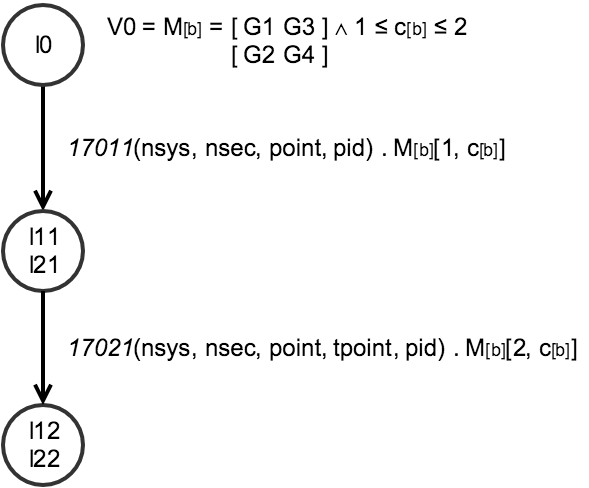
\includegraphics[width=0.5\linewidth]{figures/STS2.png}
    \end{center}

	\caption{Reduced Symbolic Transition System model obtained
    from the model depicted in Figure \ref{fig:firstmodel}.}
	\label{fig:reduced-model}
\end{figure}

Figure \ref{fig:reduced-model} depicts the reduced model obtained
from the STS of Figure \ref{fig:firstmodel}. Now we have only one
branch where guards are packed into one matrix $M_{[b]}$.

Given a STS $\EuScript{S}_i$, every STS branch is initially
adapted to express sequences of guards in a vector form to ease
the STS reduction. Later, the concatenation of these vectors
shall give birth to matrices. This adaptation is obtained with
the definition of the STS operator $Mat$:

\begin{definition}[The $Mat$ operator]
\label{rule:matrix}
  Let $\EuScript{S}_i=<L_{\EuScript{S}_i},l0_{\EuScript{S}_i},V_{\EuScript{S}_i},V0_{\EuScript{S}_i},I_{\EuScript{S}_i},\Lambda_{\EuScript{S}_i},$
  $\rightarrow_{\EuScript{S}_i}>$ be a STS. We denote by
  $Mat(\EuScript{S}_i)$ the STS operator which consists in
  expressing guards of STS branches in a vector form.

  $Mat(\EuScript{S}_i)=<L_{Mat(\EuScript{S}_i)},l0_{Mat(\EuScript{S}_i)},V_{Mat(\EuScript{S}_i)},V0_{Mat(\EuScript{S}_i)},I_{Mat(\EuScript{S}_i)},\Lambda_{Mat(\EuScript{S}_i)},$
  $\rightarrow_{Mat(\EuScript{S}_i)}>$ where:

	\begin{itemize}
    \item $L_{Mat(\EuScript{S}_i)}=L_{\EuScript{S}_i}$;
    \item $l0_{Mat(\EuScript{S}_i)}=l0_{\EuScript{S}_i}$;
    \item $I_{Mat(\EuScript{S}_i)}=I_{\EuScript{S}_i}$;
    \item $\Lambda_{Mat(\EuScript{S}_i)} = \Lambda_{\EuScript{S}_i}$;

    \item $V_{Mat(\EuScript{S}_i)}$, $V0_{Mat(\EuScript{S}_i)}$
      and $\rightarrow_{Mat(\EuScript{S}_i)}$ are given by the
      following rule:

    \begin{center}
    {\Large
    $\frac{b_i=l0 \xRightarrow{(a_1(p_1),G_1,A_1)...(a_n(p_n),G_n,A_n)} l_n}{
      \begin{matrix}
        V0_{Mat(\EuScript{S}_i)}:=V0_{Mat(\EuScript{S}_i)} \wedge M_{i}=[G_1,...,G_n]\\
        l0_{Mat(\EuScript{S}_i)} \xRightarrow{(a_1(p_1),M_i[1],id_V) ...(a_n(p_n),M_i[n],id_V) }_{\rightarrow_{Mat(\EuScript{S}_i)}} l_n\\
      \end{matrix}
    }$
    }
    \end{center}
  \end{itemize}

  Given a branch $b_i \in (\rightarrow_{Mat(\EuScript{S}_i)})^n$,
  we also denote by $Mat(b_i)=M$ the vector used with $b_i$.
\end{definition}

Now, we are ready to merge the STS branches that have the same
sequences of actions. This last sentence can be interpreted as an
equivalence relation over STS branches from which we can derive
equivalence classes:

\begin{definition}[STS branch equivalence class]
Let
$\EuScript{S}_i=<L_{\EuScript{S}_i},l0_{\EuScript{S}_i},V_{\EuScript{S}_i},V0_{\EuScript{S}_i},I_{\EuScript{S}_i},\Lambda_{\EuScript{S}_i},$
$\rightarrow_{\EuScript{S}_i}>$ be a STS obtained from
$Traces(Sua)$ (and having a tree structure). $[b]$ denotes the
equivalence class of $\EuScript{S}_i$ branches such that: $[b]=\{
b_j= l0_{\EuScript{S}_i}\\
\xRightarrow{(a_1(p_1),G_{1j},A_{1j})\dots(a_n(p_n),G_{nj},A_{nj})}
l_{nj}(j\geq 1) \mid b=l0_{\EuScript{S}_i}
\xRightarrow{(a_1(p_1),G_{1},A_{1})\dots(a_n(p_n),G_{n},A_{n})}
l_n\}.$
\end{definition}

The reduced STS denoted by $R(\EuScript{S}_i)$ of
$\EuScript{S}_i$ is obtained by concatenating all the branches of
each equivalence class $[b]$ found in $Mat(\EuScript{S}_i)$ into
one branch. This is achieved by an algorithm based on hashes (cf.
Section \ref{sec:impl-exp-collect}). The vectors found in the
branches of $[b]$ are concatenated as well into the same unique
matrix $M_{[b]}$. A column of this matrix represents a complete
and ordered sequence of guards found in one initial branch of
$\EuScript{S}_i$. $R(\EuScript{S}_i)$ is defined as follow:

\begin{definition}[Reduced STS $R(\EuScript{S}_i)$]
	\label{rule:min}

	Let $\EuScript{S}_i=<L_{\EuScript{S}_i},l0_{\EuScript{S}_i},V_{\EuScript{S}_i},V0_{\EuScript{S}_i},I_{\EuScript{S}_i},\Lambda_{\EuScript{S}_i},$ $\rightarrow_{\EuScript{S}_i}>$ be
    a STS inferred from a structured trace set $Traces(Sua)$. The reduction of $\EuScript{S}_i$ is modeled by the STS
	$R(\EuScript{S}_i)= <L_R,l0_R,V_R,V0_R,I_R,\Lambda_R,$
	$\rightarrow_R>$ where:

  \begin{center}
      {\Large
  $\frac{\begin{matrix}
      [b]=\{b_1,...,b_m\},
      b=l0_{\EuScript{S}_i} \xRightarrow{(a_1(p_1),G_{1},A_{1})...(a_n(p_n),G_{n},A_{n})}_{Mat(\EuScript{S}_i)} l_{n}\\
    \end{matrix}
  }
  {\begin{matrix}
      V0_R:=V0_R \wedge M_{[b]}=[Mat(b_1),...,Mat(b_m)] \wedge (1 \leq c_{[b]} \leq m),\\
      l0_R \xRightarrow{(a_1(p_1),M_{[b]}[1,c_{[b]}],id_V)... (a_n(p_n),M_{[b]}[n,c_{[b]}],id_V)}_{\rightarrow_R}\\  (l_{n1}...l_{nm})
    \end{matrix}
  }$
  }
  \end{center}
\end{definition}

The resulting model $R(\EuScript{S}_i)$ is a STS composed of
variables assigned to matrices whose values are used as guards. A
matrix column represents a successive list of guards found in a
branch of the initial STS $\EuScript{S}_i$. The choice of the
column in a matrix depends on a new variable $c_{[b]}$.

Figure \ref{fig:firstmodel} has two branches that can be combined
since they have the same action sequences. During the
construction of the reduced STS depicted in Figure
\ref{fig:finalmodel}, the guards are placed into two vectors
$M1=[G1\text{ }G2]$ and $M2=[G3\text{ }G4]$.  These are combined
into the same matrix $M_{[b]}$. The variable $c_{[b]}$ is used to
take either the guards of the first column or the guards of the
second one.

\begin{figure}[ht]
  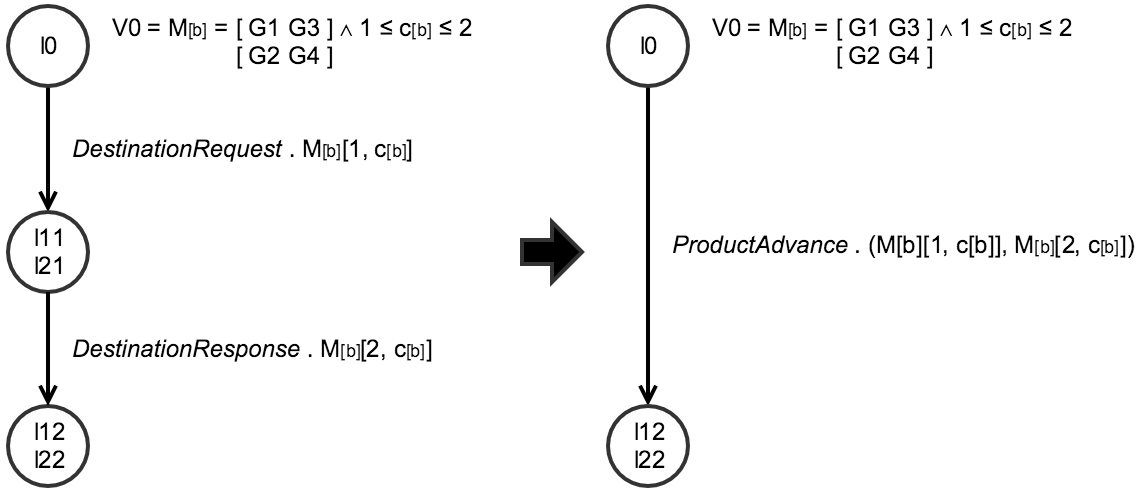
\includegraphics[width=1.0\linewidth]{figures/STSfinal.png}

    \caption{The construction of the final Symbolic Transition
    System model. The final model is on the right, obtained after
    having applied all abstraction rules.}
	\label{fig:finalmodel}
\end{figure}

The STS $R(\EuScript{S}_i)$ has less branches but still expresses
the initial behaviors described by the STS $\EuScript{S}_i$.
$R(\EuScript{S}_i)$ and $\EuScript{S}_i$ are said trace
equivalent \cite{petrenko06}.  This is captured by the following
proposition:

\begin{proposition}
  Let $\mathit{Sua}$ be a system under analysis and $Traces(Sua)$ be its traces
  set. $R(\EuScript{S}_i)$ is a STS derived from $Traces(Sua)$.
  We have $Traces(R(\EuScript{S}_i)) = Traces(\EuScript{S}_i) =
  CTraces(Sua) \subseteq Traces(Sua)$.
\end{proposition}

\subsection{STS abstraction}

Given the trace set $ST_i \in CTraces(Sua)$, the generated STS
$R(\EuScript{S}_i)$ can be used for analysis purpose but is still
difficult to manually interpret, even for experts.  This fifth
\textit{Autofunk} module aims to analyze $R(\EuScript{S}_i)$ in order to
produce a new STS $\EuScript{S}_i^\uparrow$ whose level of
abstraction is lifted by using more intelligible actions. This
process is performed with inference rules, which encode the
knowledge of the expert of the system. These are triggered on the
transitions of $R(\EuScript{S}_i)$ to deduce new transitions. We
consider the same two types of rules as in
\crossref{sec:modelinf:webapps}{sec:modelinf:webapps:L4}:

\begin{itemize}
    \item the rules replacing some transitions by more
    comprehensive ones. These rules are of the form: \textit{When
    Transition $l_1 \xrightarrow{a(p),G,A}_{R(\EuScript{S}_i)}
    l_2$, condition on $a(p),G,A$, Then add $l_1
    \xrightarrow{a'(p'),G',A'}_{\EuScript{S}_i^\uparrow} l_2$ and
    retract $l_1 \xrightarrow{a(p),G,A}_{R(\EuScript{S}_i)}
l_2$};

    \item the rules that aggregate some successive transitions
    to a single transition compound of a more abstract action.
    These rules are of the form \textit{When Transition $l_1
    \xRightarrow{(a_1,G_1,A_1),...(a_n,G_n,A_n)} l_n$, condition
    on $(a_1,G_1,A_1),...(a_n,G_n,A_n)$, Then add $l_1
    \xrightarrow{a(p),G,A}_{\EuScript{S}_i^\uparrow} l_n $, and
    retract $l_1 \xRightarrow{(a_1,G_1,A_1),...(a_n,G_n,A_n)} l_n$}.
\end{itemize}

The generated STSs represent recorded scenarios modeled at a
higher level of abstraction. These can be particularly useful for
generating documentation or better understanding how the system
behaves, especially when issues are experienced in production.
On the other hand, it is manifest that the trace inclusion
property is lost with the STSs constructed by this module since
sequences are modified.

\begin{figure}[ht]
\begin{framed}
\begin{BVerbatim}
rule "Mark destination requests"
when:
  $t: Transition(action == "17011")
then
  $t.setAction("Destination Request")
end
\end{BVerbatim}
\end{framed}

\begin{framed}
\begin{BVerbatim}
rule "Mark destination responses"
when:
  $t: Transition(action == "17021")
then
  $t.setAction("Destination Response")
end
\end{BVerbatim}
\end{framed}

  \caption{Two rules adding value to existing transitions by
  replacing their actions by more intelligible ones. These names
  are part of the domain language used by Michelin experts.}
  \label{rule:rename-tr}
\end{figure}

\begin{figure}[ht]
\begin{framed}
\begin{BVerbatim}
rule "Aggregate destination requests/responses"
when
  $t1: Transition(
    action == "Destination Request", $lfinal := Lfinal
  )
  $t2: Transition(
    action == "Destination Response" , Linit == $lfinal
  )
then
  insert(
    new Transition(
      "Product Advance",
      Guard( $t1.Guard, $t2.Guard),
      Assign($t1.Assign, $t2.Assign),
      $t1.Linit,
      $t2.Lfinal
    )
  )
  retract($t1)
  retract($t2)
end
\end{BVerbatim}
\end{framed}

  \caption{An inference rule that aggregates two transitions of a
  Symbolic Transition System into a single transition. An example
  of its application is given in Figure \ref{fig:finalmodel}.}
  \label{rule:aggregate-tr}
\end{figure}

If we take back our example, the actions of the STS of Figure
\ref{fig:reduced-model} are replaced with the rules of Figure
\ref{rule:rename-tr} that change the labels $17011$ and
$17021$ to more intelligible ones. The third rule of
Figure \ref{rule:aggregate-tr} aggregates the two transitions
into a unique transition indicating the movement of a product in
its production line. $Transition$ are facts modeling STS
transitions as seen in Chapter \ref{sec:modelinf:webapps}. We
need a variable $\$lfinal$ that retains the final location of the
first transition $\$t1$, so that we can reuse it in the condition
of the second transition $\$t2$. The final location of the first
transition must be the initial location of the second transition
($Linit == \$lfinal$) to perform the aggregation.
From 5 initial production events that are not self-explanatory,
we generate a simpler STS constituted of one transition, clearly
expressing a part of the functioning of the system.

% By writing 20 rules to enrich the meaning of the actions for our
% case study with Michelin, we were able to generate a model that
% Michelin experts understood. We then wrote 6 more rules to
% aggregate sequences of transitions in order to generate reduced
% models, mimicking some of the existing Michelin specifications.

%%%%%%%%%%%%%%%%%%%%%%%%%%%%%%%%%%%%%%%%%%%%%%%%%%%%%%%%%%%%%%%%%

\section{Implementation and experimentation}
\label{sec:modelinf:prodsystems:results}

In this section, we briefly describe the implementation of our
model inference framework for Michelin. Then, we give an
evaluation on real production systems.

\subsection{Implementation}
\label{sec:impl-exp-collect}

Our framework \textit{Autofunk} is developed in Java and leverages Drools.
In our industrial context, we have several bases of facts used
throughout the different \textit{Autofunk} modules, represented as Java
objects such as: Events, Trace sets $ST_i$, Runs, Transitions,
and STSs. We chose to target performance and simplicity while
implementing \textit{Autofunk}. That is why most of the steps are
implemented with parallel algorithms (except the production event
parsing). Figure \ref{fig:autofunk_initial_setup} shows the
initial setup of \textit{Autofunk}. We have sets of log files to parse
coming from Michelin's logging system. \textit{Autofunk} reads these
files, and transforms them into traces, that are then used to
build models.

\begin{figure}[ht]
    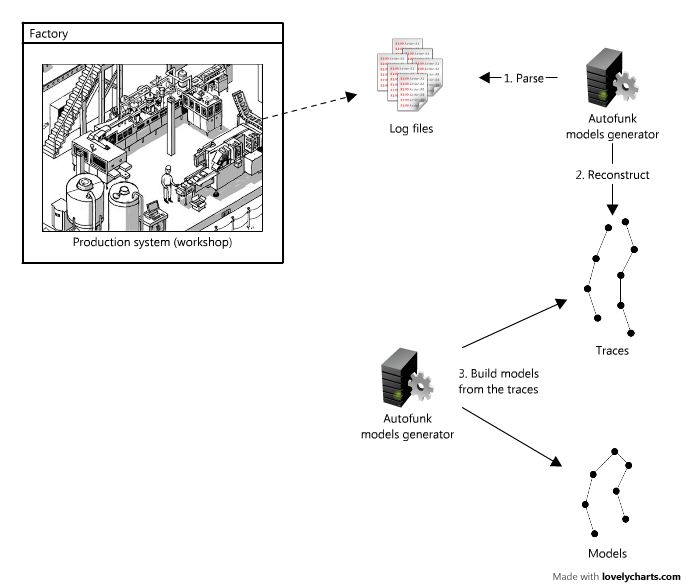
\includegraphics[width=1.0\linewidth]{figures/autofunk_initial_setup.png}

    \caption{The architecture of \textit{Autofunk} that has been
        used to conduct our first experiments with Michelin log
        files. A newer (and better) architecture is given in
        Figure \ref{fig:autofunk_gen_branded}.}
    \label{fig:autofunk_initial_setup}
\end{figure}

The input trace collection is constructed with a classical
parser, which returns $Event$ Java objects. By now, we are not
able to parallelize this part because of an issue we faced with
Michelin's logging system. The resulting drawback is that the
time to parse traces is longer than expected and heavily depends
on the size of data to parse. The $Event$ base is then filtered
with Drools inference rules as presented in Section
\ref{part3:collecting}.  Then, we call a straightforward
algorithm for reconstructing traces: it iterates over the $Event$
base and creates a set for each assignment of the identifier
$pid$. These sets are sorted to construct traces given as $Trace$
Java objects. These objects correspond to $Traces(Sua)$. The
generation of the trace subsets $ST= \{ST_1,...,ST_N\}$ and of
the first STSs are done with Drools inference rules applied in
parallel.

The STS reduction, and specifically the generation
of STS branches equivalence classes, has been implemented with a
specific algorithm for better performance. Indeed, comparing
every action in STS branches in order to aggregate them is time
consuming.  Given a STS $\EuScript{S}$, this algorithm generates
a signature for each branch $b$, \emph{i.e.} a hash
(SHA1\footnote{Secure Hash Algorithm 1} algorithm) of
the concatenation of the signatures of the actions of $b$. The
branches which have the same signature are gathered together and
establish branch equivalence classes (as described in Section
\ref{sec:modelinf:prodsystems:reduction}). Implementing
equivalence classes using hashes allows to quickly reduce STS of
any size, especially because this technique scales well.
Thereafter, the reduced $R(\EuScript{S})$ is constructed thanks
to the inference rule given in Section
\ref{sec:modelinf:prodsystems:reduction}.

At the time of writing, we are working on the architecture
depicted in Figure \ref{fig:autofunk_gen_branded}. It shows how
we plan to integrate \textit{Autofunk} with any Michelin
production system.  Events are collected on-the-fly from a system
under analysis, and sent to a database
(Elasticsearch\footnote{\url{https://www.elastic.co/products/elasticsearch}}
here) thanks to a message broker (namely
RabbitMQ\footnote{\url{https://www.rabbitmq.com/}}). Initial
benchmarks revealed that such an infrastructure allows to collect
up to 10,000 events per second with a negligible overhead on the
system. \textit{Autofunk} then queries the database to fetch
product events, and finally build models. This approach also
solves the issue mentioned previously. Furthermore, it allows to
leverage the data for other purposes, \emph{e.g.}, visualization or more
extensive analyses.

\begin{figure}[ht]
    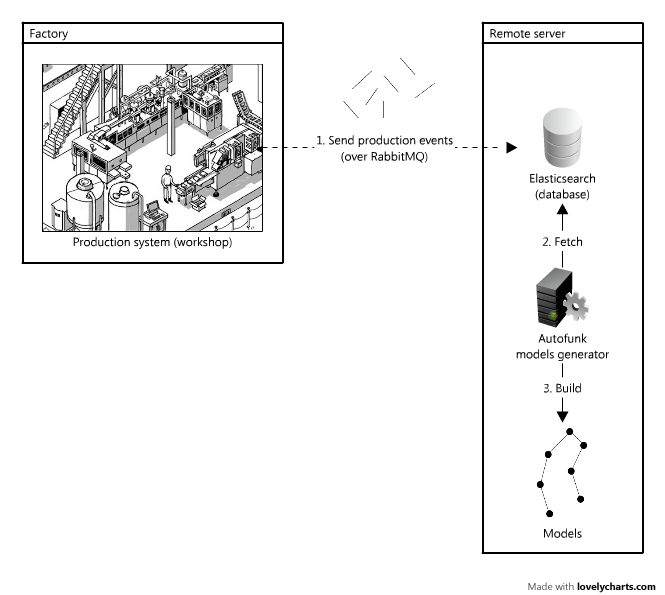
\includegraphics[width=1.0\linewidth]{figures/model-gen-branded.png}

    \caption{The overall architecture built at Michelin to use
    \textit{Autofunk} in a production environment. Events are
    sent over RabbitMQ to another server in order to minimize
    the overhead. Collected events are stored in a database.
    \textit{Autofunk} can then fetch these events, and build
    the models.}
    \label{fig:autofunk_gen_branded}
\end{figure}

\subsection{Evaluation}

We conducted several experiments with real sets of production
events, recorded in one of Michelin's factories at different
periods of time. We executed our implementation on a Linux
(Debian) machine with 12 Intel(R) Xeon(R) CPU X5660 @ 2.8GHz and
64GB RAM.

We present here the results of 6 experiments on the same
production system with different event sets collected during 1,
8, 11, 20, and 23 days. These results are depicted in Table
\ref{fig:results}. The third column gives the number of
production events recorded on the system. The next column shows
the trace number obtained after the parsing step.  $N$ and $M$
represent the entry and exit points automatically computed with
the statistical analysis. The column Trace Subsets shows how
$Traces(Sua)$ is segmented into subsets $\{ST_1,...,ST_N\}$ and
the number of traces included in each subset. These numbers of
traces also correspond to the numbers of branches generated in
the STSs $\EuScript{S}_1,...,\EuScript{S}_N$. The eighth column,
\# $R(\EuScript{S}_i)$, represents the number of branches found
in each reduced STSs $R(\EuScript{S}_1),...,R(\EuScript{S}_N)$.
Finally, execution times are rounded and expressed in minutes in
the last column.

\begin{sidewaystable}
\begin{center}
\begin{tabular}{| c | c | c | c | c | c | c | c | c | c | c |}
\hline
Experiment & Number of days & Number of events &
$Card(Traces(Sua))$ & $N$ & $M$ & \# Trace subsets & \#
$R(\EuScript{S}_i)$ & Exec. time (min)\\
\hline
\hline
$A_1$ & 1     & 660,431   & 16,602  & 2 & 3 & 4,822  & 332   & 1 \\
$A_2$ &       &           &         &   &   & 1,310  & 193   &   \\
\hline
$B_1$ & 8     & 3,952,906 & 66,880  & 3 & 3 & 28,555 & 914   & 9 \\
$B_2$ &       &           &         &   &   & 18,900 & 788   &   \\
$B_3$ &       &           &         &   &   &  6,681 &  51   &   \\
\hline
$C_1$ & 11    & 3,615,215 & 61,125  & 3 & 3 & 28,302 & 889   & 9 \\
$C_2$ &       &           &         &   &   & 14,605 & 681   &   \\
$C_2$ &       &           &         &   &   &  7,824 &  80   &   \\
\hline
$D_1$ & 11    & 3,851,264 & 73,364  & 2 & 3 & 35,541 & 924   & 9 \\
$D_2$ &       &           &         &   &   & 17,402 & 837   &   \\
\hline
$E_1$ & 20    & 7,635,494 & 134,908 & 2 & 3 & 61,795 & 1,441 & 15 \\
$E_2$ &       &           &         &   &   & 35,799 & 1,401 &    \\
\hline
$F_1$ & 23    & 9,231,160 & 161,035 & 2 & 3 & 77,058 & 1,587 & 21 \\
$F_2$ &       &           &         &   &   & 43,536 & 1,585 &    \\
\hline
\end{tabular}
\end{center}

\caption{This table shows the results of 6 experiments on a
Michelin production system with different event sets.}
\label{fig:results}
\end{sidewaystable}

First, these results show that our framework can take millions of
production events and still builds models quickly (20 minutes).
With sets collected during one day up to one week (experiments
$A$, $B$, $C$, and $D$), models are inferred in less than 10
minutes. Hence, \textit{Autofunk} can be used to quickly infer
models for analysis purpose or to help diagnose faults in a
system. Experiment $F$ handled almost 10 million events in less
than half an hour to build two models including around 1,600
branches. As mentioned in Section \ref{sec:impl-exp-collect}, the
parsing process is not parallelized yet, and it took up to 20
minutes to open and parse around 1,000 files (number of Michelin
log files for this experiment). This issue is solved by the
architecture presented in Figure \ref{fig:autofunk_gen_branded}.
The graph shown in Figure \ref{fig:time-vs-messages} summarizes
the performances of our framework, and how fast it is at
transforming production events into models (experiments $B$, $C$
and $D$ run in about 9 minutes). It also demonstrates that
doubling the event set does not involve doubling its execution
time. The linear regression reveals that the overall framework
scales well, even with the current parsing implementation.

In Table \ref{fig:results}, the difference between the number of
trace subsets (7th column) and the number of branches included in
the STSs $R(\EuScript{S}_i)$ (8th column) clearly shows that our
STS reduction approach is effective. For instance, with
experiment $B$, we reduce the STSs by 91.88\% against the initial
trace set $Traces(Sua)$. In other words, 91\% of the original
behaviors are packed into matrices. As a reminder, such results
are tied to the specific context of Michelin production systems.
The reduction ratio may vary with other systems.

\begin{figure}[ht]
  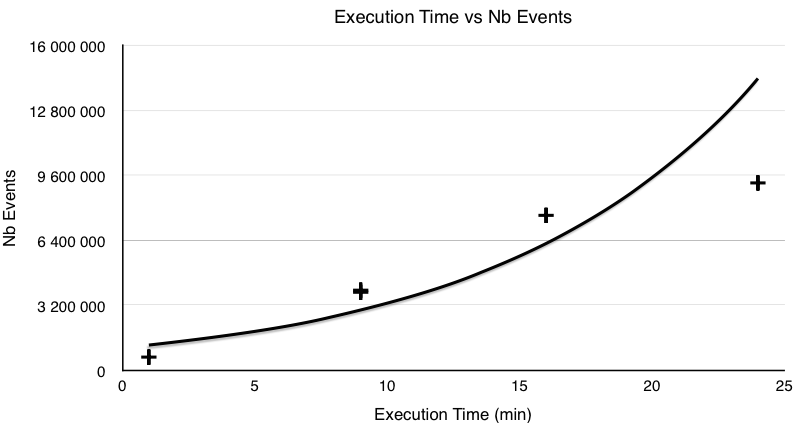
\includegraphics[width=1.0\linewidth]{figures/time-vs-messages.png}

  \caption{Execution time vs events. According to the trend shown
  by the linear regression, we can state that our framework
  scales well.}
  \label{fig:time-vs-messages}
\end{figure}

We also extracted the values of columns 4 and 7 in Table
\ref{fig:results} to depict the stacked bar chart illustrated in
Figure \ref{fig:proportions}. This chart shows, for each
experiment, the proportion of complete traces kept by
\textit{Autofunk} to build models, over the initial number of
traces in $Traces(Sua)$.  \textit{Autofunk} has kept only 37\% of
the initial traces in Experiment $A$ because its initial trace
set is too small and contains many incomplete behaviors. During a
day, most of the recorded traces do not start or end at entry or
exit points, but rather start or end somewhere in production
lines (cf. Section \ref{prodsys:context}). That is why, on a
single day, we can find so many incomplete traces. With more
production events, such a phenomenon is limited because we absorb
these storage delays.

\begin{figure}[ht]
  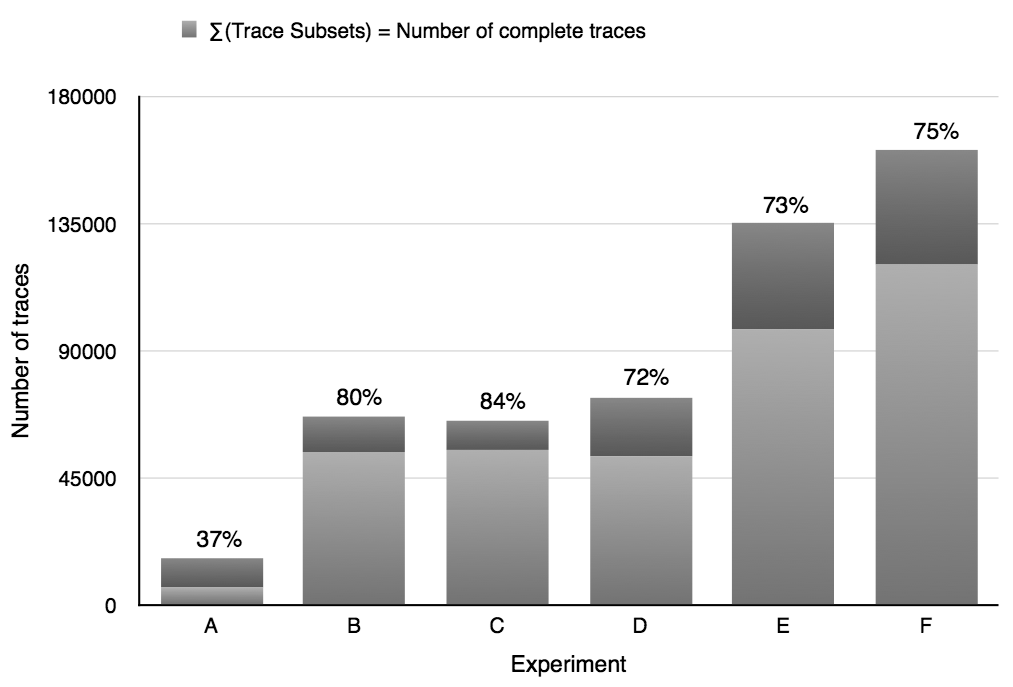
\includegraphics[width=1.0\linewidth]{figures/proportions.png}

  \caption{Proportions of complete traces for the different
  experiments. This chart shows that \textit{Autofunk} considers
  a lot of traces to infer models, but there is still room for
  improvement.}
  \label{fig:proportions}
\end{figure}

We can also notice that experiments $C$ and $D$ have similar
initial trace sets but experiment $C$ owns more complete traces
than experiment $D$ by 12\%, which is significant. Furthermore, experiments
$B$ and $C$ take 3 entry points into account while the others only
take 2 of them. This is related to the fixed limit of 10\% we
chose to ensure truly entry points to be automatically selected.
The workshop we analyzed has three entry points whose two are
mainly used. The third entry point is employed to balance the
production load between this workshop and a second one located
close to it in the same factory. Depending on the period, this
entry point may be more or less solicited, hence the
difference between experiments $B$, $C$ and experiment $D$.
Increasing the limit of 10\% to a higher value would change the value
of $N$ for experiments $B$ and $C$, but would also impact
experiment $A$ by introducing false results since incorrect entry
points could be selected. By means of a manual analysis, we
concluded that 10\% was the best ratio for removing incomplete
traces in our experiments.  30\% of initial traces have been
removed, which is close to the reality.

Another potential issue with our parsing implementation is that
every event has to be loaded in memory, so that we can perform
computation and apply our algorithms on them. But working
with millions of Java objects requires a lot of memory, \emph{i.e.}
memory consumption depends on the amount of initial traces. We
compared execution time and memory consumption in Figure
\ref{fig:memory-time}, showing that memory consumption tends to
follow a logarithmic trend. In the next version of
\textit{Autofunk}, we plan to work on improving memory
consumption even if it has been considered acceptable as is by
Michelin.

\begin{figure}[ht]
  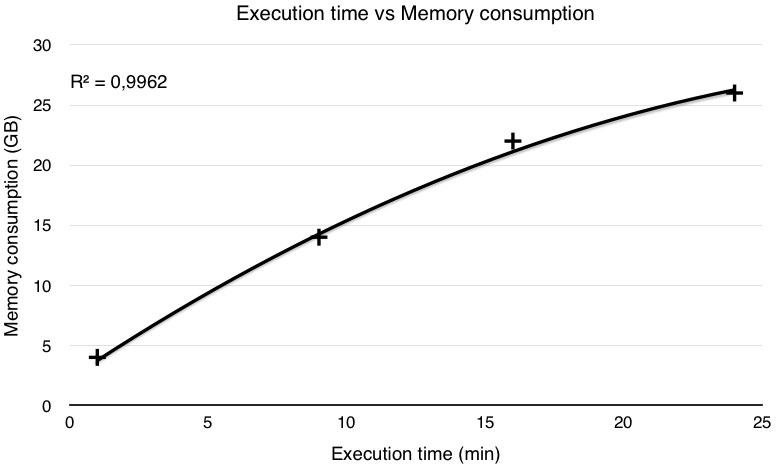
\includegraphics[width=1.0\linewidth]{figures/memory-time.png}

  \caption{Execution time vs memory consumption. This version 2 of
  \textit{Autofunk} is still a prototype, and memory consumption
  remains an issue.}
  \label{fig:memory-time}
\end{figure}

For confidentiality reasons, we are not able to provide results
related to the generation of more abstract models.

%%%%%%%%%%%%%%%%%%%%%%%%%%%%%%%%%%%%%%%%%%%%%%%%%%%%%%%%%%%%%%%%%

\section{A better solution to the trace segmentation and
filtering problem with machine learning}
\label{sec:modelinf:prodsystems:better-segmentation}

In Section \ref{sec:modelinf:prodsystems:segmentation}, we
presented a statistical analysis to segment and filter the
initial trace set used to infer models, part of \emph{Autofunk
v2}. Nevertheless, experiments (as seen in the previous section)
revealed that this empirical method was not stable, in other
words the use of a configurable minimum limit was not accurate
enough. That is why we chose to work on a new solution to segment
and filter traces, which gave birth to \emph{Autofunk v3}.

\emph{Autofunk v3} now relies on a \emph{machine learning}
technique to segment a trace set into several subsets, one per
entry point of the system $\mathit{Sua}$. We leverage this
process to also remove incomplete traces, \emph{i.e.} traces that
do not express an execution starting from an entry point and
ending to an exit point. These can be extracted by analyzing the
traces and the variable $point$, which captures the product
physical location.

In order to determine both entry and exit points of
$\mathit{Sua}$, we rely on an outlier detection approach
\cite{1695852}. An outlier is an observation that deviates so
much from the other observations as to arouse suspicions that it
was generated by a different mechanism. More precisely, we chose
to use the \emph{k-means clustering} method
\cite{10.2307/2346830}, a machine learning algorithm, which is
both fast and efficient, and does not need to be trained before
being effectively used (that is called unsupervised learning, and
it is well-known in the machine learning field). \textit{k-means
clustering} aims to partition $n$ observations into $k$ clusters
as shown in Figure \ref{fig:kmeans}.

\begin{figure}[ht]
    \begin{center}
        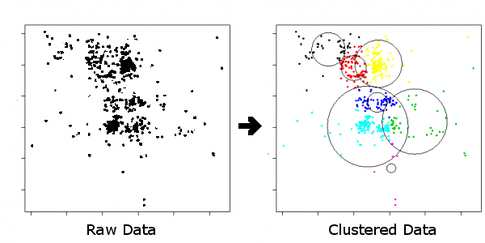
\includegraphics[width=1.0\linewidth]{figures/kmeans.png}
    \end{center}

    \caption{k-means clustering explained: the intuition is to
    partition $n$ observations into $k$ clusters in which each
    observation belongs to the cluster with the nearest mean.}
    \label{fig:kmeans}
\end{figure}

In our context, observations are represented by the variable
$point$ present in each trace of $Traces({Sua})$, which captures
the product physical location, and $k=2$ as we want to group the
outliers together, and leave the other points in another cluster.
But, since we want to leverage the largest part of the initial
trace set, we apply \textit{k-means clustering} several times
until reaching 80\% of traces retained in a cluster.

Once the entry and exit points are found, we segment
$Traces({Sua})$ and obtain a set $CTraces({Sua})=\{ST_1, \dots,
ST_n\}$. Then, we apply the same generation and reduction steps
as described in Section \ref{sec:modelinf:prodsystems:generation}
and Section \ref{sec:modelinf:prodsystems:reduction} so that we
obtain the reduced model $R(\EuScript{S}) =
\{R(\EuScript{S}_1),\dots,R(\EuScript{S}_n)\}$.

%%%%%%%%%%%%%%%%%%%%%%%%%%%%%%%%%%%%%%%%%%%%%%%%%%%%%%%%%%%%%%%%%

\section{Conclusion}
\label{sec:modelinf:prodsystems:conclusion}

In this chapter, we presented our revisited framework
\textit{Autofunk}, combining model inference, machine learning,
and expert systems to generate models from production systems.
Figure \ref{fig:autofunk_branded} shows the final architecture of
our \emph{third} version of \textit{Autofunk} along with the
technologies used in each module. Given a large set of production
events, our framework infers exact models whose traces are
included in the initial trace set of a system under analysis
\cite{petrenko06}.  We chose to design \textit{Autofunk} for
targeting high performance. Our evaluation shows that this
approach is suitable in the context of production systems since
we quickly obtain STS trees reduced by 90\% against the original
trace sets of the system under analysis.

\begin{figure}[h]
    \begin{center}
        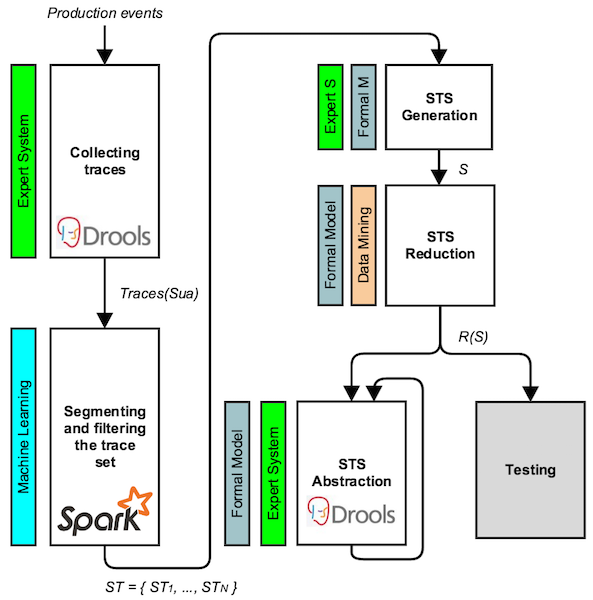
\includegraphics[width=1.0\linewidth]{figures/autofunk_branded.png}
    \end{center}

    \caption{Final architecture of our framework \textit{Autofunk},
    designed for quickly inferring models of Michelin's production systems.}
    \label{fig:autofunk_branded}
\end{figure}

While there is still room for improvement on how we generate
exact models, we decided to go deeper and use such models for
testing purpose. In the next chapter, we describe our testing
technique that leverages the work presented in this chapter.
